\section{Experiments}

\subsection{Death Avoidance Decomposition}
\label{sec:death-decomp}

\begin{figure}[t]
\centering
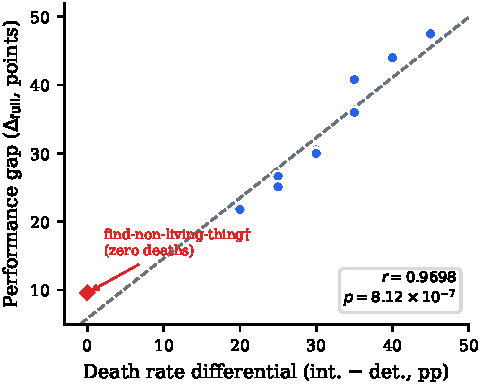
\includegraphics[width=\columnwidth]{fig1_daf_scatter.pdf}
\caption{Per-task death rate differential (internal minus deterministic) vs.\ $\Delta_{\text{full}}$. Each point represents one of 11 task types. Regression: $r = 0.9698$ ($p = 8.12 \times 10^{-7}$).}
\label{fig:decomposition}
\end{figure}

The full performance gap between deterministic and internal strategies across 245 episodes is $\Delta_{\text{full}} = +29.60$ points. Excluding all episodes where either strategy results in death, the gap collapses to $\Delta_{\text{nd}} = +2.84$. The resulting DAF (\S\ref{sec:daf}) is 90.41\%: approximately 90\% of the deterministic strategy's advantage is attributable to death avoidance.

This concentration is consistent across task types (Appendix~\ref{app:per-task}). The Pearson correlation between per-task death rate differential and $\Delta_{\text{full}}$ is $r = 0.9698$ ($p = 8.12 \times 10^{-7}$; Figure~\ref{fig:decomposition}). The internal strategy dies in 42.9\% of episodes versus 16.3\% for deterministic---a 2.6$\times$ ratio driving the bulk of the score difference.

The label distribution reflects this asymmetry: 86 \texttt{det\_preferred}, 9 \texttt{internal\_preferred}, 150 \texttt{no\_preference}. When internal reasoning does not cause death, it performs comparably to deterministic computation.

One task reveals residual non-death signal: \texttt{find-non-living-thing} ($n=40$) has zero deaths yet $\Delta_{\text{full}} = +9.58$, entirely from non-death differences. Among the 10 death-prone task types, however, death avoidance overwhelms non-death signal.

\subsection{Baselines}
\label{sec:baselines}

\begin{table}[t]
\centering
\small
\begin{tabular}{@{}lccc@{}}
\toprule
Strategy & Score & 95\% CI & Death \% \\
\midrule
Always-Internal & $-39.07$ & [$-46.40$, $-32.27$] & 42.9 \\
Always-Det. & $-9.47$ & [$-14.71$, $-4.29$] & 16.3 \\
Random & $-22.38$ & [$-28.67$, $-15.75$] & 27.8 \\
Oracle & $-6.58$ & [$-11.54$, $-1.70$] & 14.3 \\
\midrule
Trained Router & $-10.70$ & [$-16.33$, $-5.27$] & 17.6 \\
\bottomrule
\end{tabular}
\caption{Episode-weighted mean scores on ScienceWorld (11 task types, 245 episodes). 95\% Bootstrap CIs. The oracle selects the higher-scoring strategy per episode; 96.3\% of its decisions match always-deterministic.}
\label{tab:baselines}
\end{table}

Table~\ref{tab:baselines} reports episode-weighted mean scores and death rates. Always-deterministic ($-9.47$) outperforms always-internal ($-39.07$) by 29.60 points, consistent with $\Delta_{\text{full}}$. The oracle improves only modestly to $-6.58$, with 96.3\% of its decisions matching always-deterministic---\emph{oracle degeneracy} indicating the optimal routing policy closely resembles unconditional deterministic computation. Random routing ($-22.38$) falls between the two pure strategies.

Keyword-based routing fails: ScienceWorld's generic action verbs cause match rates to cluster at extremes (85.8\% or $<$5\%), degenerating to a pure strategy.

The trained router (\S\ref{sec:router-diagnostic}) scores $-10.70$, 1.23 points below always-deterministic, with comparable death rate (17.6\% vs.\ 16.3\%).

\subsection{Router Training as Diagnostic}
\label{sec:router-diagnostic}

We investigate whether episode-level counterfactual labels can train a step-level router, as a diagnostic probe rather than a routing system proposal.

\paragraph{Classification head.} A linear head appended to the LLM's hidden representations degenerates to always-deterministic (0\% internal recall) across all configurations (class weighting, focal loss, undersampling, temperature scaling).

\paragraph{Implicit router.} We fine-tune Qwen3-1.7B to internalize routing decisions. With GA=8 (effective batch 32), the model achieves 65.4\% generation accuracy and 51.5\% internal recall---the only non-degenerate configuration. GA=1 reaches 74.5\% logit accuracy but only 53.3\% generation accuracy (26.7\% internal recall)---a 21.2pp logit--generation gap indicating batch size governs transfer to generation.

Across four seeds (GA=8), balanced accuracy is $58.1 \pm 0.8\%$ (8 points above chance), with internal recall ranging 51.5--81.8\%. End-to-end, the router invokes the simulator 97.0\% of the time (Table~\ref{tab:baselines})---consistent with minimal routing structure beyond death avoidance.
